\section{Approach}
\label{sec:approach}


In our method, the summary can be represented by different topics. Each topic 
is a distribution over words. We get the probability $p(w|t)$ of the word 
given topic of all words in summary in sequence and generate a linear sequence 
on each topic. This sequence can represent the summary on corresponding topic. 
The length of it is the number of words in corresponding summary. In the other word, 
the summary is a set of linear sequence on different topics. The number of the 
linear sequence in one summary is as the same as the number of topics. We use 
LDA to get the number of the topics and the probabilistic values. 

We have two methods to evaluate the similarity between system summary 
and model summaries. One is a probabilistic framework. The other is 
a weighted model.

Let $Sim(s,m,t)$ be the similarity between system summary 
$s$ and model summary $m$ on the topic $t$. We use $Score(s,M)$ as the score of the
system summary $s$ and model summaries set $M$ by our approach.

\subsection{Probabilistic Framework}

At first, we will describe the Probabilisitc Framework used in our method.

Let $s$ be the system summary, $M$ be a set of model summaries, $m$ be the model 
summary, $c$ be the number of the model summaries, $t$ be a topic from 
a set of $T$ all topics, $W_{s}$ be the set of words in system summary, 
$W_{m}$ be the set of words in model summary, $w$ be the word of all words in summary.
We model the quality of the system summary as a probability of generate the system 
summary $s$ given the set of model summaries $M$:

\begin{eqnarray*}
p(s | M) &=& \frac{\sum_t p(s, M, t)}{p(M)} \\
	&=& \frac{\sum_t\prod_m p(m, t) p(s | m, t)}{p(M)} \\
	&=& \frac{\sum_t\prod_m p(m, t) p(s | m, t)}{\prod_m p(m)} \\
	&=& {\sum_t\prod_m p(m | t) p(s | m, t)} \\
	&=& {\sum_t\prod_m p(W_{m} | t) p(s | m, t)} \\
        &=& {\sum_t\prod_m\prod_w p(w | t) p(s | m, t)}\\
\end{eqnarray*}

We can get the Score(s,M) function:

\begin{equation*}
Score(s,M) = p(s|M) 
\end{equation*}

$p(s|m,t)$ is the equivalent to Sim(s,m,t).

In the weighted model, we give a weight to the similarity on each topic
between system summary and model summaries. Let $weight_{t}$ be the weight 
on the topic $t$. The weight indicate the importance of the topic in the 
model summaries. Because we use the probability sequence as the summary.
So, we can describe the summary use a graph, for example: 

\KZ{Give a system summary graph and a model summary graph.}
\begin{figure}[th]
\center
\epsfig{file=D1113-1.eps,width=0.4\columnwidth,angle=270}
\caption{System summary D1113-1}
\label{fig:digit}
\end{figure}

The percentage of the area of the shadow part shows the important of the model summary
on one topic. It is represented the weight on this topic.

\begin{equation*}
Score(s,M) = \frac{\sum_m\sum_t weight_{t} Sim(s,m,t)}{c}
\end{equation*}


\subsection{Ordinal Similarity}

We use three methods to calculate the similarity between system summary 
probalilistic sequence and model summary probalilistic sequence on the same topic. 
One is Dynamic time warping(DTW). The other two are about rank correlation 
coefficients, such as Spearman's rank correlation coefficient and Kendall's 
rank correlation coefficient.

According to the definition of DTW, any data which can be represented as 
a linear sequence  can be analyzed with DTW. In our idea, Each summary 
on one topic can be represented as a linear sequence, 
which is called word series.

Suppose there are two word series identifying system summary sequence and 
model summary sequence on one topic, $s$ and $m$, of length $Ls$ and $Lm$,
$ws_{i}$ and $wm_{j}$ is the $i_{th}$ of the words in system summary and model summary,
where:
\begin{eqnarray*}
s &=& ws_{1},ws_{2},...,ws_{i},...,ws_{Ls}\\ 
m &=& wm_{1},wm_{2},...,wm_{j},...,wm_{Lm} 
\end{eqnarray*}
For example:
\KZ{Give the graph of sequence system and model summary on one topic.}

First, we construct an s-by-m matrix where the value of the $(i, j)$ element 
is the distance $dist(i,j)$ between the two points $ws_{i}$ and $wm_{j}$:

\begin{equation*}
dist(i,j) = ws_{i}-wm_{j}
\end{equation*}

For example:
\KZ{Give an example for the distance matrix based on system and model summary on one topic.}
 
A warping path D is a contiguous set of matrix elements that defines
a mapping between $s$ and $m$. The k is the index of the element of D. 
So we have:

\[D = d_{1},d_{2},...,d_{k},\]
where $\max \left\{ Ls, Lm\right\} \leq k < Ls + Lm - 1$.

In our method, we need to know which path has the lowest warping cost. 
By using dynamic programming,  we can find this path. We construct a new s-by-m matrix 
where the value of the $(i,j)$ elements is the cumulative distance $dtw(i,j)$ as 
the distance $dist(i,j)$ and the minimum of the cumulative distances of 
the adjacent elements:

\begin{equation*}
dtw(i,j) = dist(i,j)+\\
          \min \left\{ dtw(i-1,j-1),dtw(i-1,j),dtw(i,j-1)\right\}
\end{equation*}

So, the correspoding similarity function is:

\begin{equation*}
Sim(s,m,t) = dtw(Ls,Lm)
\end{equation*}

The examples in summary:
\KZ{Give an example for the cumulative matrix based on system and model summary on one topic.}

In statistics, a rank correlation coefficient measures the similarity between two rankings. 
The sequence of the p(w|t) on one topic in a summary, which is called word series above, 
can also be represented as a ranking consist of the importance of the words. This sequence 
shows the probability distrubution on one topic. The length of the sequence is the number 
of the words in the summary. 

We can use rank correlation coeffiecient to get the similarity between the system summary 
sequence and the model sumamry sequence on the same topic. However, both of Spearman 
correlation  and Kendall's correlation need two variables have the same length. 
So, we use a sampling method to get the same lenght variables. 

Suppose there is a system summary sequence and a model summary sequence on one topic, 
$s$ and $m$, of length $Ls$ and $Lm$ where:
\begin{eqnarray*}
s &=& ws_{1}, ws_{2},...,ws_{i},...,ws_{Ls} \\
m &=& wm_{1}, wm_{2},...,wm_{j},...,wm_{Lm} 
\end{eqnarray*}

We get a fixed number of subsequence from summary which length is $\max \left\{Ls,Lm\right\}$ 
with random sample. The order between the elements in the subsequence must be 
in consistent with the order between the same elements in the summary sequence. 
We set a parameter $k$ as the number of subsequence. We will get $k$ subsequence. 
Then, we calculate the average of the similarity $r$ between each subsequence and the summary 
which length is $\min \left\{Ls,Lm\right\}$. This average value is the similarity between system summary
and model summary on one topic.

The correspoding similarity function based on Spearman is:

\begin{equation*}
Sim(s,m,t) = \frac {\sum_k r}{k}
\end{equation*}

For example:
\KZ{Give an example for the two different length summary.}

Spearman's rank correlation coefficient is a nonparametric measure of rank correlation.
Spearman's rank is the covariance of the two variables divided by the product of 
their standard deviations. It evaluate the relationship between two variables. 
The values in the variable should be replaced by the ranking of the values,
such as that (0.1,0.2,0.3,0.4) should be changed to (1,2,3,4). When the two values 
of the variables are same, their ranking is obtained by averaging them, 
such as (0.1,0.2,0.2,0.4) should be changed to (1,2.5,2.5,4).
The Spearman correlation between two variables will be from -1 to 1. 
`1' means that they are identical. `-1' means that they are fully opposed. 
The higher score they get, the more similar they are.

Kendall's correlation is similar to Spearman's correlation. Compared with 
the Spearman correlation, the Kendall correlation is not affected by how far 
from each other ranks are but only by whether the ranks between variables are 
equal or not.

Let $r_{S}$ be the Spearman's correlation, $r_{K}$ be the Kendall's correlation, 
$X$ and $Y$ be the variables we will compare, $X_{i}$ and $Y_{i}$ be the ith elements
of the corresponding sequence, ${rg} (X_{i})$ and ${rg} (Y_{i})$ be the ranking of X and Y,
$n$ be the length of the variables, $d$ is the difference between the two ranks of each variables:

\begin{equation*}
r_{S} = {1-{\frac {6\sum_i d_{i}^{2}}{n(n^{2}-1)}}}
\end{equation*}

where

\begin{equation*}
d_{i} = {rg}(X_{i})-{rg}(Y_{i})
\end{equation*}

For example:
\KZ{Give an example for Spearman's correlation.}

For kendall's correlation,($ x_{1}$, $y_{1}$), ($x_{2}$, $y_{2}$), …, ($x_{n}$, $y_{n}$) 
is a set of observations of the joint random variables $X$ and $Y$ respectively, 
such that all the values of $x_{i}$ and $y_{i}$ are unique. 
Any pair of observations ($x_{i}$, $y_{i}$) and ($x_{j}$, $y_{j}$), where $i\not=j$, 
are said to be concordant if the ranks for both elements agree: 
if both $x_{i} \ge x_{j}$ and $y_{i} \ge y_{j}$ or if both $x_{i} \le x_{j}$ and $y_{i} \le y_{j}$. 
They are said to be discordant, if $x_{i} \ge x_{j}$ and $y_{i} \le y_{j}$ or 
if $x_{i} \le x_{j}$ and $y_{i} \ge y_{j}$. If $x_{i}=x_{j}$ or $y_{i}= y_{j}$, the pair is neither 
concordant nor discordant.

There are three method to calculate Kendall's tau. There may be the same values in 
variables so that we should use the tau-b as our calculate function $r_{K}$:

\begin{equation*}
r_{K} = {\frac {n_{c}-n_{d}}{\sqrt {(n_{0}-n_{1})(n_{0}-n_{2})}}}
\end{equation*}

where
\begin{eqnarray*}
n_{0}&=&n(n-1)/2\\
n_{1}&=&\sum_i t_{i}(t_{i}-1)/2\\
n_{2}&=&\sum_j u_{j}(u_{j}-1)/2\\
n_{c}&=&{\text{Number of concordant pairs}}\\
n_{d}&=&{\text{Number of discordant pairs}}\\
\end{eqnarray*}

tau-b range from −1 to +1 like Spearman's correlaiton. `0' indicates the absence of association.

For example:
\KZ{Give an example for kendall's correlation.}

The probabilistic framework is based on a Topic-word Models.
\subsection{Topic-word Models}
To model $p(w, t)$. 
LDA, word embedding. Discuss the corpuses we use. How to preprocess 
the data, etc.

By using this model, each topic is a distribution over words. Each word in summaries 
can also be represented as a N-dimentional vector of topics. For our analysis, 
we describe the summaries as a matrix specifies the probability $p(w|t)$ of words given topic. 
In addition, we use the probability $p(t|w)$ of topic given words to indicate the importance of 
one topic in each words.

Example:
1.\KZ{Give a example for probability p(w|t)}
2.\KZ{Give a example for probability p(t|w)}
